\documentclass[12pt, landscape]{article}
\usepackage[scaled=0.92]{helvet}
\usepackage{multicol}
\usepackage{calc}
\usepackage{ifthen}
\usepackage[landscape]{geometry}
%\usepackage{hyperref}

\usepackage{newtxtext} 

%for strikeout
\usepackage{ulem}

%For editing parbox
\usepackage[table]{xcolor}
%For editing itemise margins, reduce iterm separaion and list separation
\usepackage{enumitem}
% For math
\usepackage{amsmath,amsthm,amsfonts,amssymb}

%For pictures / figures
\usepackage{color,graphicx,overpic}
\graphicspath{ {./images/} }

%\usepackage{newtxtext} 
%\usepackage{amssymb}
%\usepackage[table]{xcolor}
%\usepackage{vwcol}
%\usepackage{tikz}
%\usepackage{wrapfig}
%\usepackage{makecell}

% Create cases
\usepackage{mathtools}

% Template: Cheatsheet with code enabled

%--------------------------- PACKAGES ABOVE --------------------------------------------------------------

\pdfinfo{
  /Title (ST2334.pdf)
  /Creator (Ger Teck)
  /Author (Ger Teck)
  /Subject ()
  /Keywords (tex)}

%% Margins for PAPER

% This sets page margins to .5 inch if using letter paper, and to 1cm
% if using A4 paper. (This probably isn't strictly necessary.)
% If using another size paper, use default 1cm margins.
\ifthenelse{\lengthtest { \paperwidth = 11in}}
	{ \geometry{top=.5in,left=.5in,right=.5in,bottom=.5in} }
	{\ifthenelse{ \lengthtest{ \paperwidth = 297mm}}
		{\geometry{top=1cm,left=1cm,right=1cm,bottom=1cm} }
		{\geometry{top=1cm,left=1cm,right=1cm,bottom=1cm} }
	}

% Turn off header and footer
\pagestyle{empty}

% for tight centres (less spacing)
\newenvironment{tightcenter}{%
  \setlength\topsep{0.5pt}
  \setlength\parskip{0.5pt}
  \begin{center}
}{%
  \end{center}
}

% Redefine section commands to use less space
\makeatletter
\renewcommand{\section}{\@startsection{section}{1}{0mm}%
                                {-1ex plus -.5ex minus -.2ex}%
                                {0.5ex plus .2ex}%x
                                {\normalfont\large\bfseries}}
\renewcommand{\subsection}{\@startsection{subsection}{2}{0.1mm}%
                                {-1explus -.5ex minus -.2ex}%
                                {0.5ex plus .2ex}%
                                {\normalfont\normalsize\bfseries}}
\renewcommand{\subsubsection}{\@startsection{subsubsection}{3}{0.1mm}%
                                {-1ex plus -.5ex minus -.2ex}%
                                {1ex plus .2ex}%
                                {\normalfont\small\bfseries}}
% change font
%\renewcommand{\familydefault}{\sfdefault}
%\renewcommand\rmdefault{\sfdefault}
\linespread{1.05}

\makeatother

% Define BibTeX command
\def\BibTeX{{\rm B\kern-.05em{\sc i\kern-.025em b}\kern-.08em
    T\kern-.1667em\lower.7ex\hbox{E}\kern-.125emX}}

% Don't print section numbers
\setcounter{secnumdepth}{0}

\setlength{\parindent}{0pt}
\setlength{\parskip}{0pt plus 0.5ex}

%% this changes all items (enumerate and itemize, reduce margins)
\setlength{\leftmargini}{0.5cm}
\setlength{\leftmarginii}{0.5cm}
\setlist[itemize,1]{leftmargin=2mm,labelindent=1mm,labelsep=1mm, itemsep = 1mm}
\setlist[itemize,2]{leftmargin=4mm,labelindent=1mm,labelsep=1mm, itemsep = 1mm}
\itemsep = 0mm
\setlist{nosep}

% Need Logo Picture
%Watermark Top Right
%\usepackage{atbegshi,picture}
%\AtBeginShipout{\AtBeginShipoutUpperLeft{%
 % \put(\dimexpr\paperwidth-1.2cm\relax, -1.2cm){\makebox[0pt][r]{\framebox{
\includegraphics[width = 0.3cm]{mountainbooks} Ger Teck}}}%
%}}


% -------------------------------------------------------------------------------

% START OF DOCUMENT HERE

\begin{document}
\raggedright
\footnotesize
\begin{multicols*}{3}



% multicol parameters
% These lengths are set only within the two main columns
%\setlength{\columnseprule}{0.25pt}
\setlength{\premulticols}{1pt}
\setlength{\postmulticols}{1pt}
\setlength{\multicolsep}{1pt}
\setlength{\columnsep}{2pt}

%% DOCUMENT NAME HERE
\begin{center}
     \Large{\textbf{ST2334 Summary Notes}} \\
\end{center}

AY23/24 Sem 1, github.com/gerteck

\section{1. Basic Probability Concepts }
\begin{itemize}
\item \textbf{Sample Space: $S$} All possible outcomes of stat. expt.
\item \textbf{Null Event}: Event that contains no element, empty set, $\varnothing$
\item \textbf{Axioms of Probability}:  \\ 
For any event X, $0 \leq P(X) \leq 1$.  $P(S) = 1$. \\
If $A \cap B = \emptyset$ (Mut Excl), $P(A \cup B) = P(A) + P(B)$. 
\item Finite sample space with equally likely outcomes: $P(A)$ = ($\frac{\# sample points A}{\#total sample points S}$). (e.g. birthday problem)
\end{itemize}

\subsubsection{Event Operation \& Relationships}
\begin{itemize}
\item \textbf{Event Operations:} Union, Intersection, Complement.
\item \textbf{Event Relationships:} Contained: {$A \subset B$} \\
Equivalence: {$A \subset B$ with $A \supset B \rightarrow A = B$} \\
Mutually Exclusive: {$A \cap B = \emptyset$}.
\item \textbf{De Morgan's Law:} {$(A \cup B)' = A' \cap B'$} and  {$(A \cap B)' = A' \cup B'$}
\end{itemize}

\subsubsection{Counting Methods}
\begin{itemize}
\item Multiplication Principle: (Sequential Events)
\item Addition Principle: (Pairwise Disjoin sets)
\item \textbf{Permutation}: {$_{n}P_{r} = \frac{n!}{(n-r)!}$}
\item \textbf{Combination}: {$\binom{n}{r} = \frac{n!}{(n-r)!r!}$}
\end{itemize}

\subsubsection{Conditional Probability}
• Understand conditional as reduced sample space. \\
\[P(B|A) = \frac{P(B \cap A)}{P(A)} = \frac{P(A|B)P(B)}{P(A)}\]

\subsubsection{Independence}
$A \perp B \leftrightarrow P(A \cap B) = P(A)P(B)$ \\
$A \perp B \leftrightarrow P(A|B) = P(A)$

% \vfill \null
\columnbreak


\subsubsection{Law of Total Probability}
\begin{itemize}
\item \textbf{Partition: }{If $A_1, \cdots, A_n$ mutually exclusive, $\bigcup _{i=1} ^{n} A_i = S$, then $A_1, \cdots, A_n$ are partitions.}
 \item If $A_1, \cdots, A_n$ are partitions of S, then for any event B:
    \[P(B) = \sum _{i=1} ^{n} P(B \cap A_i) = \sum _{i=1} ^{n} P(B|A_i)P(A_i)\]
\end{itemize}

\subsubsection{Bayes' Theorem}
Let $A_1, \cdots, A_n$ be partitions of S. For any event B:
\[P(A_k|B) = \frac{P(B|A_k)P(A_k)}{\sum _{i=1} ^{n} P(B|A_k)P(A_i)}\] 
For when $n = 2$, $\{A, A' \}$ becomes a partition of $S$.
\[P(A|B) = \frac{P(A)P(B|A))}{P(A)P(B|A) + P(A')P(B|A')}\] 

\section{2. Random Variables}
A function X, which assigns a real number to every s $\in$ S is
called a random variable. \\
• \textbf{Range space}: $Rx = \{x|x = X(s), s \in S\}$ \\
• Likewise, the set X $\in$ A, for A being a subset of R, is also a subset of $S: {s \in S : X(s) \in A}$.


\subsubsection{Probability Distribution}
Two main types of RV used in practice: discrete and continuous.
\begin{itemize}
    \item Probability assigned to each possible $X$
    \item Given RV $X$ with range of $R_x$:
        \subitem \textbf{Discrete: }{Numbers in $R_x$ are finite or countable}
        \subitem \textbf{Continuous: }{$R_x$ is interval}
\end{itemize}

\subsubsection{(Discrete) Probability Mass Function $f(x)$:}
\[
f(x)
    \begin{cases*}
        P(X=x), & for $x\in R_X$ \\
        0, & for $x\notin R_X$\\
    \end{cases*}
\]
\begin{enumerate}
	\item $f(x_i) = P(X = x_i) \geq 0$ for $x_i \in R_x$
      \item $f(x_i) = 0$ for $x_i \notin R_x$
      \item $\sum _{i=1} ^{\infty} f(x_i) = 1$ (PSum = 1)
      \item $\forall B \subseteq \mathbb{R}, P(X \in B) = \sum _{x_i \in B \cap R_x} f(x_i)$
\end{enumerate}

\subsubsection{(Continuous) Probability Density Function $f(x)$:}
\begin{itemize}
    \item {Given $R_x$ is interval. Quantifies probability that $X$ is in some range.}
    \item $p.f.$ must satisfy:
        \begin{enumerate}
            \item $f(x) \geq 0$, $f(x) = 0$ for $x \notin R_x$
            \item No need $f(x) \leq 1$ (Concerned with area)
            \item $\int _{R_x} f(x) dx = 1$ (Integration over $R_X$ = 1)
            \item $\forall a,b \text{ s.t. } a \leq b, P(a \leq X \leq b) = \int _{a} ^{b} f(x) dx$
        \end{enumerate}
    \item \textbf{Note:} $P(X = x_0) = \int _{x_0} ^{x_0} f(x) dx = 0$
    \item Hence, to check if a function is a pdf, \\
    	 1. $f(x) \geq 0$  for $x \in R_x$,  $f(x) = 0$ for $x \notin R_x$ \\
    	 2. $\int _{R_x} f(x) dx = 1$.
\end{itemize}

\subsection{Cumulative Distribution Function}
Describes distribution of a RV $X$: cumulative distribution function (cdf), applicable for discrete or continuous RV.
\[F(x) = P(X \leq x)\]
 $F(x)$ is non-decreasing and $0 \leq F(x) \leq 1$ \\
• Probability fn \& cumulative distribution fn have one-to-one correspondence. For any probability fn given, the cdf is uniquely determined, vice versa.

\subsubsection{CDF Discrete RV: Step Function $F(x)$}

    \[F(x) = \sum _{t \in R_x; t \leq x} f(t)\]
	\centerline{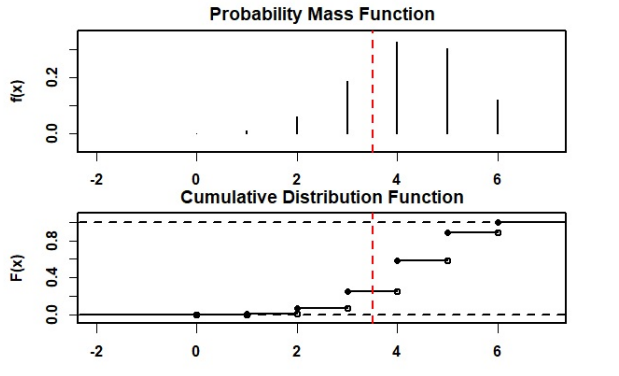
\includegraphics[width=0.5\linewidth]{cdfstep}}
    \begin{itemize}
       \item $P(a \leq X \leq b)=P(X \leq b)-P(X < a)$
       \item $P(a \leq X \leq b)=F(b)-F(a-)$
	\item $P(a \leq X \leq b) =  F(b) - \lim _{x \to a^-} F(x)$
       \item $0 \leq f(x) \leq 1$
       \item  c.d.f has to be \textbf{right continuous} (• ---)
    \end{itemize}

%\vfill \null
\columnbreak

\subsubsection{CDF Continuous RV: $F(x)$}
    \[F(x) = \int _{-\infty} ^{x} f(t) dt\]
    \[impt: f(x) = \frac{d(F(x))}{dx}\]
    \centerline{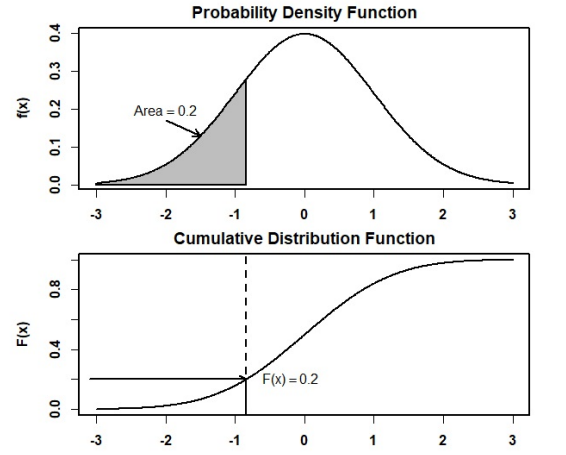
\includegraphics[width=0.5\linewidth]{cdfcontinuous}}
    \begin{itemize}
        \item $P(a \leq X \leq b) = P(a < X < b) = F(b) - F(a)$
        \item $0 \leq f(x)$. \\
         e.g. $f(x) = 3x^2$ is a valid $p.f.$ since $\int _{R_x} f(x) dx = 1$
    \end{itemize}
    
   
\subsection{Expectation $\mu$ \& Variance $\sigma$}
\subsubsection{Expectation of Random Variable: $\mu$ }
\begin{itemize}
    \item \textbf{Mean of discrete RV}: 
    \[\mu = E(X) = \sum _{x \in R_x} x_i f(x_i) = \sum _{i=1} ^{\infty} P(X \geq i)\]
    \item \textbf{E.g.}: X discrete RV with p.m.f. $f(x)$ and range $R_X$ \\ 
     $\mu =$ $E(g(x)) = \sum _{x \in R_x} g(x)f(x)$
    
    \medskip
    \item \textbf{Mean of continuous RV}: 
    \[\mu = E(X) = \int _{x \in R_x} x f(x) dx\]
    \item \textbf{E.g.}: X continuous RV with p.d.f. $f(x)$ and range $R_X$ \\
    $\mu =$ $E(g(x)) = \int _{x \in R_x} g(x)f(x)dx$
    
    \smallskip
    \item \textbf{Properties of Expectation:}
    \item $E(aX + b) = aE(X) + b$
    \item Linearity of expectation: $E(X + Y) = E(X) + E(Y)$
\end{itemize}

\columnbreak

\subsubsection{Variance of Random Variable: $\sigma$}

\[\sigma_X^2 = V(X) = E[(X - \mu_X)^2]\]

\begin{itemize}
    \smallskip
    \item \textbf{Variance of discrete RV}: 
    \[V(X) = \sum _{x \in R_x} (x - \mu_X)^2 f(x)\]
    
    \medskip
    \item \textbf{Variance of continuous RV}: 
    \[V(X) = \int _{x \in R_x} (x - \mu_X)^2 f(x) dx\]
    
    \medskip
    \item $V(X) \geq 0$ and $V(X) = 0$ when $X$ is a constant
    \item $V(aX+b) = a^2V(X)$
    \item \textbf{alt. form:} $V(X) = E(X^2) - (E(X))^2$
    \item \textbf{Standard Deviation: }{$\sigma_X = \sqrt{V(X)}$}
\end{itemize}
    
    
\section{3. Joint Distributions}
\begin{itemize}
    \item Consider more than 1 RV simultaneously, 
    \item Given sample space $S$. Let $X$ and $Y$ be functions mapping $s \in S \to \mathbb{R}$: $(X, Y)$ is 2D random vector.
    \[\text{\textbf{Range spc:}} R_{X, Y} = \{(x,y) | x = X(s), y=Y(s), s \in S\}\]
    \item \textbf{Discrete 2D RV:} \\
    {\# of possible values of $(X(s), Y(s))$ finite / countable}
    \item \textbf{Continuous 2D RV}:  \\
    	{\# of possible values of $(X(s), Y(s))$ assume any value in some region of the Euclidean space $\mathbb{R}^2$}
    \item If both $X$ and $Y$ are discrete/continuous, then $(X, Y)$ is discrete/continuous respectively.
\end{itemize}

\subsection{Joint Probability Function}

\begin{itemize}
     \item \textbf{Joint Probability (mass) function, 2D discrete RV}:
    \[f_{X,Y} (x,y) = P(X = x, Y = y)\]
    \begin{itemize}
        \item $f_{X,Y} (x,y) \geq 0$ for any $(x,y) \in R_{X,Y}$
        \item $f_{X,Y} (x,y) = 0$ for any $(x,y) \notin R_{X,Y}$
        \item $\sum _{i=1} ^{\infty} \sum _{j=1} ^{\infty} P(X = x_i, Y = y_i) = 1$
        \item Let $A \subseteq R_{X, Y}$. $P((X,Y) \in A) = \sum \sum _{(x,y) \in A} f_{X, Y}(x,y)$
    \end{itemize}
     \item \textbf{Joint Probability (density) function, 2D cont. RV}:
    \[P(a \leq X \leq b, c \leq Y \leq d) = \int _a ^b \int _c ^d f_{X, Y} (x, y)dydx\]
    \begin{itemize}
        \item $f_{X,Y} (x,y) \geq 0$ for any $(x,y) \in R_{X,Y}$
        \item $f_{X,Y} (x,y) = 0$ for any $(x,y) \notin R_{X,Y}$
        \item $\int _{-\infty} ^{\infty} \int _{-\infty} ^{\infty} f_{X,Y} (x,y)dxdy = 1$ \\
        or equivalently:
        \item $\int _{} ^{} \int _{(x,y) \in R_{X,Y}} ^{} f_{X,Y} (x,y)dxdy = 1$
    \end{itemize}
\end{itemize}

\subsection{Marginal Probability Function}
Marginal distribution of $X$ is individual distribution of $X$, ignoring the value of $Y$. “Projection” of 2D function
$f_{X,Y}(x, y)$ to 1D function. \\
\medskip
Let $(X,Y)$ be 2D RV with joint probability function $f_{X,Y} (x,y)$:
\[\text{If $Y$ is \textbf{discrete}, } f_X(x) = \sum _y f_{X,Y} (x,y)\]
\[\text{If $Y$ is \textbf{continuous}, } f_X(x) = \int _{-\infty} ^\infty f_{X,Y} (x,y)dy\]

\begin{itemize}
    \item $f_Y (y)$ defined similarly
    \item $f_X(x)$ is a $p.f.$, satisfies all properties of prob. fn.
\end{itemize}

\subsection{Conditional Distribution}

Let $(X,Y)$ be 2D RV with joint probability function $f_{X,Y} (x,y)$. 
Then $\forall x$ s.t. $f_X(x) > 0$: ($X$ marg prob fn.) \\
\textbf{Conditional probability function of $Y$ given $X$ = $x$:}

\[f_{Y|X} (y|x) = \frac{f_{X,Y}(x,y)}{f_X (x)}\]

\begin{itemize}
    \item Intuition: Distribution of $Y$ given $X = x$
    \item Only defined for $x$ s.t. $f_X(x) > 0$
    \item $f_{Y|X} (y|x)$ is a $p.f.$ if we fix $x$, satisfies prop. of prob.fn.
    
    \medskip
    \item But, $f_{Y|X} (y|x)$ is not a $p.f.$ for $x$: No need for sum / integral over x = 1. Hence, \\
    	If $f_X (x) > 0$: $f_{X,Y} (x,y) = f_X (x)f_{Y|X} (y|x)$ \\
    	If $f_Y (y) > 0$: $f_{X,Y} (x,y) = f_Y (y)f_{X|Y} (x|y)$
    \item \textbf{Probability Y $\leq y$, Average $Y$ given $X = x$}
    \item $P(Y \leq y | X = x) = \int _{-\infty} ^y f_{Y|X} (y|x)dy$
    \item $E(Y|X=x) = \int _{-\infty} ^{\infty} y f_{Y|X} (y|x)dy$
\end{itemize} 
  
  
  
  
  
  
  
\end{multicols*}
\end{document}